\chapter{Tecnologías}
\label{chap:tecnologias}
\observacion{Para el desarrollo de videojuegos?}
\observacion{Una sección más al final como un resumen/tabla/gráfico del stack
    service móvil}

Luego de definir los requerimientos y el alcance \fixme{que tener}{es
    fundamental revisar las tecnologías} \fixme{la solución propuesta se deben
    seleccionar de manera}{} adecuada las tecnologías que serán utilizadas para
implementarla de tal forma que cumpla con todos los requerimientos, el esquema
general de interacción se observa en~\ref{fig:componentes}.

En este capítulo se describen en detalle estas tecnologías haciendo énfasis
especial a la selección del motor de videojuegos, el cual es la principal
herramienta requerida, por lo mismo, se describen los principales motores
utilizados en la actualidad y se definen criterios para seleccionar de entre
ellos el más adecuado.


\begin{figure}
\begin{center}
    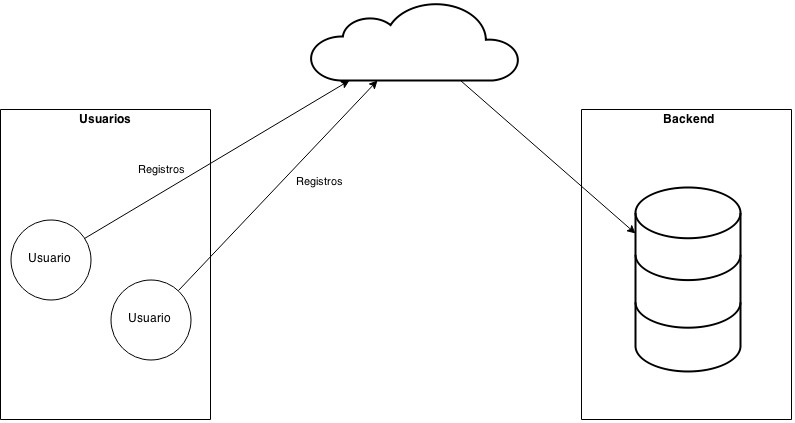
\includegraphics[scale=0.5]{tecnologias/images/completo.png}
\end{center}
\caption{Esquema general de los componentes}
\label{fig:componentes}
\end{figure}

\fixme{Entrando un poco más en detalle}{} dentro de la implementación de la
solución, se describen las herramientas que son necesarias para el desarrollo
del juego a más bajo nivel como el lenguaje de programación, herramientas para
modelado 3D, gestores de código fuente, entre otros. Estas tecnologías son
agrupadas en tres partes principales:

\observacion{Agregar footnotes para definir backend y frontend}
\begin{itemize}
    \item \textbf{Herramientas de gestión de código}: se describen las
        tecnologías requeridas para gestionar y mantener código.
    \item \textbf{Desarrollo del \textit{frontend}}: se describen aquellas tecnologías
        utilizadas para el desarrollo del videojuego en sí. El \textit{frontend} es la
        parte de la solución que interactúa con el usuario y por lo tanto es lo
        que él puede percibir.
    \item \textbf{Desarrollo del \textit{backend}}: se describen aquellas tecnologías
        utilizadas para procesar las acciones que los usuarios realizan dentro
        de la solución.
\end{itemize}

\fixme{La tecnología necesaria debe permitir crear escenarios en tres
    dimensiones, animaciones y otros aspectos relacionados a los videojuegos,
    como iluminación, interacción entre componentes, etc, además de otros
    factores importantes como comunicación, audio, etc.}{Esto no debería ir en
    frontend?}

Los factores relacionados a los videojuegos son cubiertos por un \enquote{Motor
    de videojuegos}, y los demás factores deben ser tratados con software
\fixme{especial}{?}.

Es necesario un \textit{backend} que permita almacenar la información de todos
los usuarios de tal forma a unificar el acceso a los registros de los usuarios,
esto implica que los usuarios deberán tener una conexión a Internet ocasional
para que puedan enviar los registros.

También se requiere que pueda almacenar información de todos los usuarios, con
la mayor cantidad de detalle posible, para así poder realizar análisis
posteriores. La \fixme{cantidad}{El tiempo tota por práctica} de tiempo
utilizado, cantidad de procedimientos realizados y frecuencia de uso, son
ejemplos de información que debe ser registrada para su posterior análisis.



\section{Motores de videojuegos}

Para el desarrollo de videojuegos se utilizan programas o herramientas
especializadas en ello llamadas \enquote{Motores de videojuegos}. A continuación
se da una breve introducción de lo que es un motor de videojuego.

El término \enquote{motor de videojuegos} hace referencia a una serie de rutinas
de programación que permiten el diseño, la creación, el desarrollo y la
representación gráfica de un videojuego\cite{videojuego:telechea}.

Además, la gran mayoría de estos motores ofrecen a su vez características y
funciones que facilitan la construcción del videojuego, como el motor físico
(software capaz de realizar \enquote{simulaciones} de ciertos sistemas físicos
como la dinámica de un cuerpo rígido, el movimiento de un fluido o la
elasticidad) o detector de colisiones, sonidos, \textit{scripting}, animaciones,
inteligencia artificial, comunicación a través de redes, \textit{streaming},
administración de memoria, etc\cite{videojuego:telechea}.

El motor de videojuego a utilizar depende de las características que posea el
videojuego que se quiere desarrollar, las cuales fueron descritas en
\ref{chap:requerimientos}. A continuación se da una breve descripción
de los motores de videojuegos más utilizados actualmente, se definen los
criterios de selección y se realiza una comparación entre los mismos, para la
elección del motor de videojuegos que más se adecue a las necesidades de la
solución. Entre los aspectos que son comparados se encuentran la distribución,
librerías, tiendas, licencias, curva de aprendizaje, lenguajes de programación,
entre otros.

\subsection{Unreal Development Kit}

Es la edición gratuita de \textit{Unreal Engine 3}. \textit{Unreal Engine} es el
motor de videojuegos desarrollado por \textit{Epic Games}\cite{unrealengine}.

\Gls{udk} proporciona acceso al motor de juegos 3D y a la herramienta profesional 
que se utiliza en el desarrollo de videojuegos \textit{blockbuster}, visualización 
arquitectónica, el desarrollo de juegos para móviles, modelos 3D, películas digitales 
y más. Utilizando \Gls{udk} se pueden implementar juegos y aplicaciones en
\textit{Windows PC}, \textit{iOS} y \textit{Mac}\cite{unrealengine}.

Posee su propio entorno de desarrollo, las rutinas de programación pueden ser escritas 
en los lenguajes de programación Unreal Script y C++, y una comunidad 
grande donde se puede recurrir. Además soporta formatos de modelos 
3D como fbx, dds, raw y ASE\cite{unrealengine}.

\subsection{Blender Game Engine}

\enquote{Blender Game Engine} es el motor de videojuegos de \textit{Blender Foundation} 
que permite crear aplicaciones 3D interactivas o simulaciones, desarrollado bajo 
la licencia \Gls{gnu}\cite{blender}.

\textit{Blender Game Engine} genera las escenas de forma continua en tiempo real
e incorpora facilidades para la interacción del usuario durante el proceso de
\textit{renderización}, procesa la lógica de sonido, de la física y la 
representación de simulaciones en orden secuencial\cite{blender}.

Posee la posibilidad de exportar en plataformas como
\textit{Windows, Linux y Mac OS}. También incluye básico en desarrollo para 
plataformas Android\cite{blender}.

Posee su propio entorno de desarrollo, las rutinas de programación pueden ser 
escritas en los lenguajes de programación Python y C++, y
una comunidad grande donde se puede recurrir. Además soporta formatos 3D 
como 3ds, dae, fbx, dxf\cite{blender}.

\subsection{CryEngine}

\enquote{CryEngine} es el motor de videojuegos desarrollado por \textit{Crytek}.
Existe una versión gratuita denominada \enquote{CryEngine Free SDK} con todas
las funcionalidades, esta versión esta disponible para su descarga, pero ya ha
sido descontinuada\cite{cryengine:sdk}.

Este motor de videojuegos permite exportar a plataformas como iOS y
Android\cite{cryengine}. Posee su propio entorno de desarrollo, las rutinas de
programación pueden ser escritas en los lenguajes de programación C++ y Lua, y
una comunidad de tamaño moderado donde se puede recurrir. Además sólo soporta
sus propios formatos 3D\cite{cryengine}.

\subsection{ShiVa3D}

\textit{ShiVa3D} es un motor para el desarrollo de videojuegos y aplicaciones 
3D desarrollado por ShiVa Technologies\cite{shiva}.

Un producto relacionado es el \enquote{ShiVa Server}, el cual permite el
desarrollo de aplicaciones multijugador. Las características de este servidor,
incluyen comunicación \textit{VoIp}, etc\cite{shiva}, esta es
una opción interesante para el desarrollo del \textit{backend}.

\textit{ShiVa} puede exportar juegos y aplicaciones a una cantidad variada de 
plataformas, incluyendo móviles como \textit{iOS, Android, BlackBerry y Windows
Phone}, de escritorio como \textit{Windows, Mac OS X y Linux}, los
navegadores web con soporte \textit{Flash y HTML5}, así como consolas como la
\textit{Xbox 360, PlayStation3 y Nintendo Wii}. El \Gls{ide} se ejecuta en
\textit{Windows} y \textit{Mac OS X}\cite{shiva}. 

Posee su propio entorno de desarrollo, las rutinas de programación pueden ser 
escritas en los lenguajes de programación FlowGraph y Lua, y una 
comunidad moderada donde se puede recurrir. Además sólo soporta el formato 
3D, dae\cite{shiva}.


\subsection{Unity3D}

\textit{Unity} es un motor para el desarrollo de juegos,
desarrollado por \textit{Unity Technologies}. Posee una versión pagada 
y una gratuita\cite{unity3d}.

Posee un motor de \textit{renderizado} y un flujo de trabajo para la creación 
de contenido 3D interactivo, además permite mezclar contenido 3D, 2D, sonidos 
y animaciones de manera sencilla\cite{unity3d}.

La versión gratuita permite desarrollar juegos para múltiples plataformas. 
Entre las plataformas móviles soportadas, encontramos a \textit{iOS, Andriod, 
Windows Phone 8, BlackBerry 10}, entre las plataformas de escritorio a 
\textit{Windows, Mac y Linux}, plataformas web como \textit{Internet Explorer,
    Mozzilla Firefox, Google Chrome}\footnote{Requiere un \textit{plugin} para
    el navegador que está disponible para \textit{Windows y Mac}}, y entre
plataformas de consolas a \textit{Xbox 360, Xbox One, Wii, Wii U, Nintendo
    3DS}\cite{unity3d}.

Posee su propio entorno de desarrollo, las rutinas de programación pueden ser 
escritas en los lenguajes de programación \cs{}, UnityScript y Boo, y una 
comunidad grande donde recurrir. Además soporta formatos 3D como fbx, obj, max, 
blend, dae, 3ds, dxf, MB, MA\cite{unity3d}.


%! TEX root = ../main.tex
\section{Selección del motor de videojuego}
\label{sec:seleccion_plataforma}

En esta sección se comparan los motores de videojuegos \textit{Unreal Engine,
    CryEngine, Blender Game Engine, ShiVa3D y Unity3D} según criterios relacionados 
con los requisitos que debe cumplir la solución. Estos criterios son citados a continuación, 
además, se selecciona y justifica la elección del motor de videojuego a utilizarse para 
el desarrollo de la solución propuesta.

\subsection{Criterios de selección}

Para seleccionar el motor de videojuego que se ajuste mejor
a la solución propuesta para facilitar su desarrollo y el cumplimiento de los
requisitos definidos en el capítulo~\ref{sec:requisitos}, se tuvieron en cuenta los
siguientes criterios:

\begin{itemize}
\item Licencia de uso del motor.
\item Plataformas móviles.
\item Lenguajes de programación para el desarrollo.
\item Tienda de librerías y paquetes.
\item Tamaño de la tienda de librerías y paquetes.
\item Representación en \textit{2D} y \textit{3D}.
\item Formatos de modelo \textit{3D} soportados.
\item Soporte de comunidades.
\item Entorno de desarrollo o \Gls{ide}.
\item Licencia del entorno de desarrollo.
\end{itemize}


\subsection{Comparación}

En la tabla~\ref{tab:comparacion_motores_juegos} se comparan los criterios citados 
anteriormente para cada uno de los motores teniendo en cuenta tanto aspectos técnicos 
como de aprendizaje y de uso.

Teniendo en cuenta el resultado de esta comparación y de acuerdo a los
requisitos que debe reunir la solución propuesta se elige a \textit{Unity3D}
como el motor de videojuego ideal para el desarrollo de este trabajo.

Las ventajas principales de esta elección son la cantidad de plataformas móviles
diferentes a las que se puede exportar y distribuir la aplicación ya que uno de
los ejes del trabajo es brindarle movilidad al usuario. Además, \textit{Unity}
posee una gran comunidad de desarrolladores lo cual es importante en los
momentos en el que se poseen dudas que se desean aclarar con rapidez.

\textit{Unity} posee una gran tienda donde se pueden encontrar desde modelos en
tres dimensiones y librerías de sonidos hasta librerías que ofrecen extender o
incluir funcionalidades. 

%\newgeometry{bottom=1cm}


\begin{sidewaystable}
\begin{tabulary}{\textwidth}{L|CCCCCCCC}
\toprule
Característica / Motor &
Unreal Engine          &
CryEngine              &
ShiVa3D                &
Unity3D                &
Blender Game Engine \\
\midrule
Distribución & iOS, soporta otros dispositivos en la versión comercial. &
iOs, Android & iOS, Android, Windows Phone, BlackBerry & Android, WindowsPhone,
iOs, BlackBerry & Soporte en desarrollo para Android \\ 

Tienda de librerias & Sí, en estado Alpha & No, existen tiendas de
terceros & Sí & Sí & Sí \\

Tamaño de tienda & Mediana & Mediana & Pequeña & Grande & Grande \\

Comunidad & Grande & Moderada & Moderada & Grande & Grande \\
Licencia del entorno de desarrollo & Gratuita solo para uso no comercial &
Propietaria & Propietaria & Gratuita para uso no comercial & GPL \\

Formatos soportados & fbx, dds, raw, ASE & Formatos propios & dae & FBX, OBJ,
Max, Blend, dae, 3ds, dxf, MB, MA, etc & 3ds, dae, fbx, dxf, etc \\

Licencia del motor & Versiones antiguas gratuitas para uso no comercial.
& Gratuita solo para uso no comercial & Propietaria, solamente la versión Web es
gratis & Versión limitada gratis, disponible para uso no comercial & GPL \\

Curva de aprendizaje & Compleja & Compleja & Compleja & Sencilla & Compleja \\

Lenguajes de desarrollo & Unreal Script y C++ & C++, Lua & FlowGraph
(propietario) y Lua & \cs{}, UnityScript y Boo & Python y C++ \\

\Gls{ide} & Si, propio & Sí, propio & Sí, propio & Sí, propio & Sí, propio \\
\bottomrule

\end{tabulary}
\caption{Comparacion entre motores de videojuegos}
\label{tab:comparacion_motores_juegos}
\end{sidewaystable}
%\restoregeometry



\section{Entorno de desarrollo de la solución}

Para llevar a cabo el desarrollo completo de la solución se debe recurrir a una 
gran cantidad herramientas, \textit{frameworks}, y recursos. En esta sección se 
describen estas tecnologías.

%En esta sección se describen todos las partes involucradas en el desarrollo de
%la solución propuesta. 

%La solución se compone de dos partes, la primera es la aplicación que los
%usuarios utilizan para realizar las prácticas, denominada \textit{Frontend}, y la segunda
%parte, es un servidor que se encarga de almacenar la información sobre los
%usuarios de la solución y como la utilizan, denominado \textit{Backend}.

%Primeramente se definen las herramientas de gestión de código, pues ellas son
%utilizadas tanto por la solución como por el \textit{backend}, luego se definen
%las herramientas específicas de la creación de la simulación y por último, se
%citan y describen de manera breve las herramientas utilizadas por el
%\textit{backend}.

%La idea detrás de separar la solución en \textit{Frontend} y \textit{Backend} 
%es que ambas partes de la solución se podrán mantener de forma separada sin que 
%el cambio de una afecte el funcionamiento de la otra. 

\subsection{Herramientas de gestión de código}

La gestión del código fuente desarrollado como parte de este trabajo de grado fue realizado
mediante la utilización de la herramienta de control de código fuente
\textit{Git}, \textit{Git} es un software de control de versiones distribuido,
de código abierto bajo la licencia \Gls{gnu}\cite{git}. El proveedor del
servicio \textit{Git} utilizado es \textit{BitBucket}\cite{bitbucket}, el cual
almacena repositorios \textit{Git}, la principal característica y motivación por
la cual se utiliza este servicio es que el mismo permite mantener varios
repositorios privados de manera gratuita\cite{bitbucket}.

\subsection{Desarrollo del \textit{front-end}}

El desarrollo de la solución requiere de una variedad importante de tecnologías
además del motor de videojuego, las herramientas descritas en esta sección complementan al
motor seleccionado y facilitan la creación de contenido.

En primer lugar, se utilizó el \Gls{ide} \textit{Unity Editor} para la creación de las escenas,
el \Gls{ide} \textit{MonoDevelop} y el lenguaje \cs{} para la programación de la
interacción entre los componentes de la solución.

Adicionalmente se utilizaron varias herramientas de diseño para crear
componentes 3D y 2D, \textit{Make Human} es utilizado para la creación de los
pacientes, \textit{3ds Max} permite la creación de objetos como gazas, y otros
elementos utilizados dentro de la solución. En cuanto a los gráficos 2D, se
utilizaron \textit{Photoshop}, y diversas páginas web que proveían contenido
gratuito.

\begin{itemize}

\item \textbf{Unity Editor}

El \Gls{ide} de \textit{Unity} es la herramienta en la se crean los videojuegos
o simulaciones. Este \Gls{ide} importa todos los \textit{asset}\footnote{Un
    \textit{Asset} es un paquete \textit{Unity} que puede contener modelos,
    librerias, sonidos, etc.}. Permite compilar las escenas con los terrenos,
luces, audios, personajes, física, entre otros. Se puede agregar interacción a
través de \textit{scripting}. Además se puede probar y editar en
forma simultánea los videojuegos y desplegarlos en las plataformas
elegidas\cite{unity3d}. 

Este editor es la única herramienta que permite crear escenas en \textit{Unity},
sin embargo, este \Gls{ide}, no permite la edición de código,\footnote{Existen
    \textit{Assets} que permiten la edición de código dentro del \textit{Unity
        Editor}, pero son pagas y de baja reputación} por ello se necesita un
editor externo de código.


\item \textbf{MonoDevelop}

\textit{MonoDevelop} es un \Gls{ide} de código abierto, bajo la licencia
\Gls{gnu} apoyado principalmente por la comunidad \textit{Mono}. Es el \Gls{ide}
utilizado por defecto en el desarrollo de aplicaciones para \textit{Unity3D}, el
mismo soporta varios lenguajes de programación, como \cs{},
\textit{UnityScript}, y \textit{Boo}. Es un \Gls{ide} multiplataforma que
soporta \textit{Windows} al igual que \textit{Unity3D}.

Existen otros editores que pueden ser utilizados para el desarrollo del código
fuente, pero los mismos no cuentan con el mismo nivel de integración y no son
gratuítos.\footnote{\textit{Microsoft Visual Studio} permite el mismo nivel de
    integración que \textit{MonoDevelop} con un \textit{plugin}, pero el mismo
    es de pago durante el desarrollo de la solución}

\item \textbf{\cs{}}

\textit{Unity3D} utiliza versiones limitadas\footnote{La definición del lenguaje
    es la misma, pero las librerías estándar no están completas}de tres
lenguajes de programación: \cs{}, \textit{UnityScript}, y
\textit{Boo}\cite{unity:script}. Estos lenguajes son compilados y orientados a
objetos.

Otra característica interesante es que, por el orden de compilación de los
proyectos \textit{Unity3D}, los archivos \textit{UnityScript} y \textit{Boo} son
compilados antes que los archivos \cs{}, esto provoca que, las clases
\textit{UnityScript} sean utilizables desde \cs{}, lo que no se cumple en el
caso contrario, es decir, las clases \cs{} no son accesibles desde código
\textit{UnityScript} o \textit{Boo}.

Por lo mencionado anteriormente se selecciona a \cs{} como el lenguaje de
implementación. Además, es el lenguaje con más ayuda en línea, y las
librerías no diseñadas específicamente para \textit{Unity3d} pueden ser
utilizadas. Otro factor que influye en la elección es la familiaridad de los
autores con lenguajes similares. 

\item \textbf{Herramientas de diseño}

Las herramientas utilizadas para crear modelos 3D e imágenes 2D son las siguientes:

\begin{itemize}
\item \textbf{MakeHuman}: es un software de código abierto bajo la licencia
    \Gls{agnu} para crear personajes humanos 3D. Es una herramienta diseñada
    para simplificar la creación de seres humanos virtuales utilizando una
    interfaz gráfica de usuario\cite{makehuman}. 
\item \textbf{3ds Max}: es un software privado de modelado 3D, que además posee
    herramientas para animación, simulación y renderización. Esta herramienta
    fue utilizada para crear objetos 3D que no fueran personajes humanos y para
    exportar modelos de un formato a otro que fuera compatible con
    \textit{Unity3D}\cite{3dsmax}.
\item \textbf{Photoshop}: es una herramienta de edición de gráficos 2D de
    \textit{Adobe}, permite la creación y edición de gráficos, es utilizada para
    la creación de iconos, botones y otro contenido 2D que forma parte de la
    solución.
\end{itemize}

\end{itemize}


\subsection{Desarrollo del \textit{back-end}}

Para registrar las actividades del usuario en el front-end, se necesita de un
servidor que almacene los datos de todos los usuarios y las actividades que
estos realizan dentro de la solución.

En la figura~\ref{fig:backend_diagrama} se puede observar en lineas generales
como funciona este servicio, desde el registro de actividades del usuario, la
comunicación con el \textit{back-end}, su posterior traducción y persistencia en
una base datos, así, este servicio debe proveer:

\begin{itemize}
    \item \textbf{Alta disponibilidad}: el servidor debe estar disponible en
        todo momento, cualquier día de la semana y a cualquier hora. Los
        requisitos de accesibilidad son estrictos, pues se necesita que los
        usuarios envíen datos sin inconvenientes cuando crean necesario.
    \item \textbf{Accesibilidad}: el servidor debe poder ser accesible desde
        cualquier red móvil.
    \item \textbf{Bajo costo de comunicación}: la comunicación del usuario con
        el \textit{back-end} debe ser lo menos costosa posible, pues se utilizan
        recursos del usuario.
\end{itemize}

\begin{figure}[H]
\centering
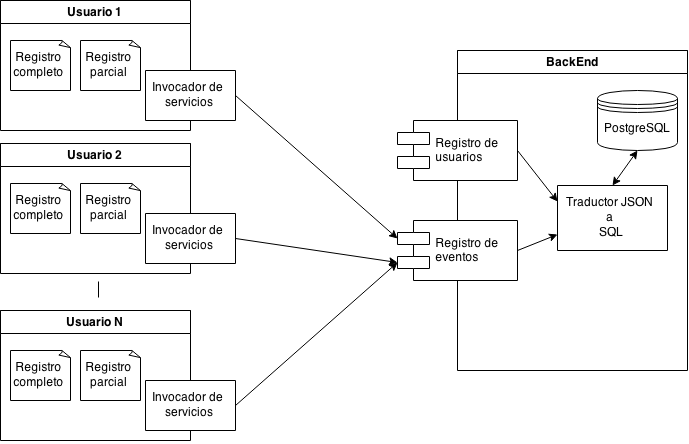
\includegraphics[scale=0.4]{tecnologias/images/backend_diagrama.png}
\caption{Diagrama de la interacción de los usuarios con el \textit{back-end}, se
    puede observar a grandes rasgos, los componentes del sistema y los servicios
    que ofrece.}
\label{fig:backend_diagrama}
\end{figure}

Las tecnologías utilizadas para el desarrollo del \textit{back-end} son:

\begin{itemize}
\item \textbf{\Gls{javaee}}

Para el desarrollo de la aplicación web que almacena los datos se utiliza
\Gls{javaee} en su versión $6$, la misma se utiliza por la familiarización de
los autores con la tecnología y la facilidad que provee para la
realización de servicios web que permitan la interacción con la solución.

\item \textbf{\Gls{rest}}

Para los servicios se utiliza la arquitectura \Gls{rest}, la principal
motivación para utilizar \Gls{rest} es la eficiencia en el uso de la
red\cite{pautasso2008restful}, la cual es también la motivación para la
utilización de \Gls{json}. La implementación del lado del servidor de la
arquitectura \Gls{rest} es \textit{RestEasy}, de parte del \textit{front-end} se utiliza
la implementación por defecto de \textit{Unity3D}.

\item \textbf{PostgresSQL}

El almacenamiento permanente de los datos se logra con la utilización de
\textit{PostgreSQL}, el cual es un motor de bases de datos de código abierto
dirigido por \textit{PostgreSQL Global
    Development Group}. La versión elegida es la $9.1$.

\item \textbf{OpenShift}

A fin de obtener las características necesarias, de alta disponibilidad y
accesibilidad, se utiliza la herramienta de plataforma como servicio de
\textit{RedHat} llamada \textit{OpenShift}, la cual es un producto de código
abierto dirigido por \textit{RedHat}.

Además de dirigir el proyecto, \textit{RedHat} provee un servicio limitado y
gratuito\cite{openshift:pricing}.\footnote{Existen versiones completas del
    producto mantenidas por \textit{RedHat}, las cuales tienen un costo mensual
    y de acuerdo a las funcionalidades utilizadas\cite{openshift:pricing}} Para
esta tesis se utilizo el servicio gratuito con la plataforma \textit{JBoss
    Application Server 7.1} y \textit{PostgreSQL 9.1}.

\end{itemize}

\section{Resumen}

A modo de resumen de las tecnologías utilizadas para el desarrollo de la solución
propuesta se presentan las tablas~\ref{tab:stack_tecnologico_fe} y~\ref{tab:stack_tecnologico_be}.

\begin{table}[H]
\centering
\begin{tabular}{lrr}
\toprule
\textbf{Utilización} & \textbf{Tecnología} & \textbf{Versión} \\
\midrule
Motor de videojuego      & Unity3d         & 4.5 \\
IDE                      & MonoDevelop     & 4 \\
                         & Unity Editor    & 4.5 \\
\midrule
Modelado 3D              & 3ds Max         & 2013 \\
Modelado 2D              & Photoshop       & 14 \\
Modelado de personajes   & MakeHuman       & 1.0 \\

\midrule
Lenguaje de programación & \cs{} \\
Gestión de código fuente & GIT & 1.8 \\
Otras librerías          & NGUI            & 2.7\\
                         & Facebook \\
                         
\bottomrule
\end{tabular}
\caption{Resumen de las tecnologías utilizadas en el \textit{front-end}}
\label{tab:stack_tecnologico_fe}
\end{table}


\begin{table}[H]
\centering
\begin{tabular}{lrr}
\toprule
\textbf{Utilización} & \textbf{Tecnología}  & \textbf{Versión} \\
\midrule
IDE                         & Eclipse & Luna\\
Lenguaje de programación    & Java & 7\\
\midrule
Servidor de aplicaciones    & Jboss & 7 \\
Servidor de base de datos   & PostgreSQL & 9.2 \\
Proveedor de plataforma     & OpenShift \\
\midrule
Gestión de código fuente    & GIT & 1.8\\
Otras librerias             & Java EE & 6\\

\bottomrule
\end{tabular}
\caption{Resumen de las tecnologías utilizadas en el \textit{back-end}}
\label{tab:stack_tecnologico_be}
\end{table}

